\paragraph{Results.} \Cref{fig:r2g,tab:r2g} show prediction accuracy.
\begin{itemize}
\item \emph{No heterogeneity ($\rho=1$).} metaBRR learns $\hat\rho\approx1$ (mean
$0.96$) and matches pooled BRR to within $0.006$ $R^2_g$ in every replicate. The extra
random effect therefore costs essentially nothing when it is not needed.
\item \emph{Increasing heterogeneity.} The advantage of metaBRR over pooled BRR grows
monotonically with $1-\rho$ and with $h^2$ (\cref{fig:gain}). Averaged over $h^2$, the
$R^2_g$ gain is $0.015$, $0.050$, $0.090$ and $0.138$ at $\rho=0.75$, $0.5$, $0.25$ and
$0$. At $h^2=0.75$ and $\rho=0.25$, metaBRR attains $R^2_g=0.365$, against $0.186$ for
pooled and $0.282$ for per-cohort BRR. At intermediate $\rho$ metaBRR beats \emph{both}
baselines: it borrows strength across cohorts for the shared component while still
fitting cohort-specific deviations.
\item \emph{No sharing ($\rho=0$).} Pooled BRR collapses to $R^2_g\approx0$, while
metaBRR learns $\hat\rho\approx0.02$ and matches per-cohort BRR exactly.
\item \emph{Heterogeneity estimation.} The estimated cross-cohort correlation $\hat\rho$
tracks the truth closely across all settings (\cref{fig:rho}). It is noisier at low
$h^2$, where there is little genetic signal to estimate it from.
\item \emph{Shared $\hat\bb_0$.} Used alone, metaBRR's $\hat\bb_0$ predicts about as
well as pooled BRR and slightly better under heterogeneity. It is the appropriate
predictor for an unseen cohort.
\end{itemize}

\begin{figure}[t]
\centering
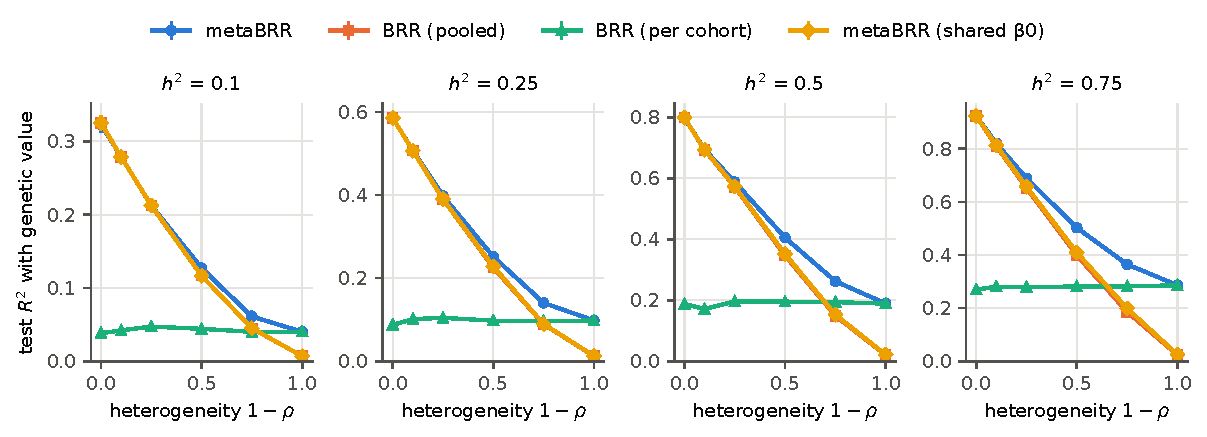
\includegraphics[width=\textwidth]{fig_r2g.pdf}
\caption{Test-set $R^2$ between predicted and true genetic value, averaged over cohorts
(mean $\pm$ s.e.\ over 3 replicates). $N=10^4$ in $K=12$ cohorts, $P=2{,}000$.}
\label{fig:r2g}
\end{figure}

\begin{figure}[t]
\centering
\begin{minipage}{0.48\textwidth}\centering
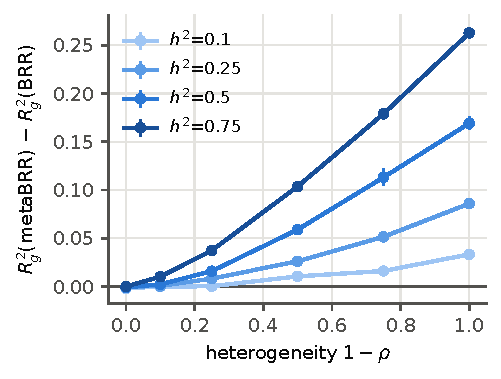
\includegraphics[width=\linewidth]{fig_gain.pdf}
\caption{Gain of metaBRR over pooled BRR in $R^2_g$.}\label{fig:gain}
\end{minipage}\hfill
\begin{minipage}{0.45\textwidth}\centering
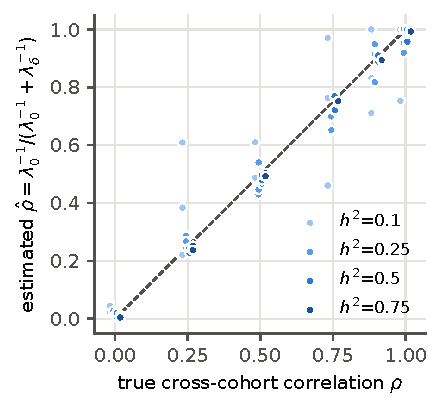
\includegraphics[width=\linewidth]{fig_rho.pdf}
\caption{Estimated vs.\ true cross-cohort correlation (each point one replicate).}\label{fig:rho}
\end{minipage}
\end{figure}

\begin{figure}[t]
\centering
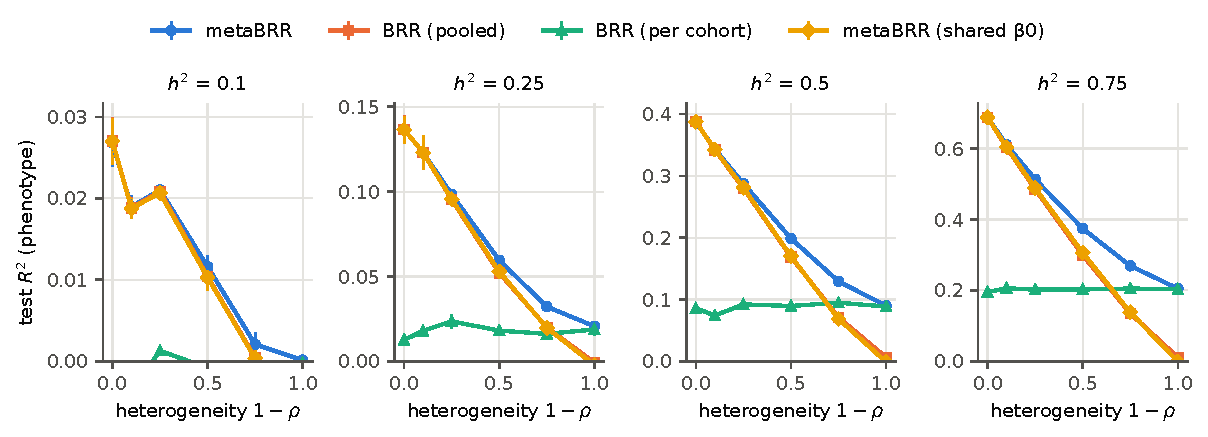
\includegraphics[width=\textwidth]{fig_r2y.pdf}
\caption{As \cref{fig:r2g}, but test-set phenotype $R^2$ (upper bound $h^2$).}
\label{fig:r2y}
\end{figure}

\begin{table}[t]
\centering\small
\caption{Mean test $R^2_g$ (best in bold).}\label{tab:r2g}
\begin{tabular}{rrcccc}
\toprule
$h^2$ & $\rho$ & BRR (pooled) & BRR (per cohort) & metaBRR (shared $\hat{\bm\beta}_0$) & metaBRR \\
\midrule
0.1 & 0 & 0.007 & \textbf{0.040} & 0.007 & 0.040 \\
0.1 & 0.25 & 0.045 & 0.040 & 0.045 & \textbf{0.061} \\
0.1 & 0.5 & 0.117 & 0.044 & 0.117 & \textbf{0.127} \\
0.1 & 0.75 & 0.212 & 0.047 & \textbf{0.213} & 0.212 \\
0.1 & 0.9 & 0.279 & 0.042 & \textbf{0.279} & 0.279 \\
0.1 & 1 & \textbf{0.325} & 0.038 & 0.325 & 0.323 \\
0.25 & 0 & 0.012 & 0.098 & 0.013 & \textbf{0.098} \\
0.25 & 0.25 & 0.089 & 0.097 & 0.090 & \textbf{0.140} \\
0.25 & 0.5 & 0.225 & 0.098 & 0.228 & \textbf{0.251} \\
0.25 & 0.75 & 0.390 & 0.104 & 0.390 & \textbf{0.398} \\
0.25 & 0.9 & 0.507 & 0.101 & 0.507 & \textbf{0.507} \\
0.25 & 1 & \textbf{0.585} & 0.088 & 0.585 & 0.585 \\
0.5 & 0 & 0.020 & 0.189 & 0.021 & \textbf{0.189} \\
0.5 & 0.25 & 0.149 & 0.194 & 0.153 & \textbf{0.262} \\
0.5 & 0.5 & 0.346 & 0.195 & 0.352 & \textbf{0.405} \\
0.5 & 0.75 & 0.572 & 0.196 & 0.573 & \textbf{0.587} \\
0.5 & 0.9 & 0.692 & 0.171 & 0.693 & \textbf{0.695} \\
0.5 & 1 & \textbf{0.798} & 0.188 & 0.798 & 0.797 \\
0.75 & 0 & 0.024 & 0.286 & 0.026 & \textbf{0.286} \\
0.75 & 0.25 & 0.186 & 0.282 & 0.199 & \textbf{0.365} \\
0.75 & 0.5 & 0.399 & 0.282 & 0.410 & \textbf{0.503} \\
0.75 & 0.75 & 0.652 & 0.278 & 0.657 & \textbf{0.689} \\
0.75 & 0.9 & 0.810 & 0.281 & 0.812 & \textbf{0.820} \\
0.75 & 1 & 0.923 & 0.270 & \textbf{0.923} & 0.923 \\
\bottomrule
\end{tabular}

\end{table}
